\documentclass[10pt,a4paper]{article}
\usepackage{amsmath}
\usepackage{amsfonts}
\usepackage{amssymb}
\usepackage{graphicx}
\usepackage[T1]{fontenc}
\usepackage[utf8]{inputenc}

\title{Grenouille}
\date {14 décembre 2018}
\author{Groupe Introduction à \LaTeX}


\begin{document}
% Let's have fun with github \o/


	\maketitle

	\section{Grenouilles dans la culture}
\subsection{Mythes bibliques}
Les grenouilles sont parfois présentes dans d'étranges phénomènes : les pluies d'animaux.

Dans la Bible, la deuxième des dix plaies d'Égypte est l'invasion des terres par des milliers de ces batraciens. 
D'après les scientifiques qui se sont penchés sur cet évènement, le phénomène pourrait s'expliquer par une sécheresse ou par l'empoisonnement des eaux du Nil.
 En effet, dans des situations de stress, ces animaux sont capables d'accélérer leur développement pour fuir plus vite leur milieu, d'où une explosion de leur nombre.

De ce fait, on peut lire dans la bible de nombreuses références négatives sur les grenouilles.
\subsubsection{Exode}
\begin{itemize}
\item 7 - 27 : Si tu refuses, toi, de le laisser partir, moi je vais infester de grenouilles tout ton territoire.
\item 7 - 28 : Le Fleuve grouillera de grenouilles, elles monteront et entreront dans ta maison, dans la chambre où tu couches, sur ton lit, dans les maisons de tes serviteurs et de ton peuple, dans tes fours et dans tes huches.
\item 7 - 29 : Les grenouilles grimperont même sur toi, sur ton peuple et sur tous tes serviteurs.
\item 8 - 1 : Yahvé dit à Moïse : Dis à Aaron : Étends ta main avec ton bâton sur les fleuves, les canaux et les marais, et fais monter les grenouilles sur la terre d'Égypte.
\item 8 - 2 : Aaron étendit la main sur les eaux d'Égypte, les grenouilles montèrent et recouvrirent la terre d'Égypte.
\item 8 - 3 : Mais les magiciens avec leurs sortilèges en firent autant, et firent monter les grenouilles sur la terre d'Égypte.
\item 8 - 4 : Pharaon appela Moïse et Aaron et dit : Priez Yahvé de détourner les grenouilles de moi et de mon peuple, et je m'engage à laisser partir le peuple pour qu'il sacrifie à Yahvé.
\item 8 - 5 : Moïse dit à Pharaon : À toi l'avantage! Pour quand dois-je prier pour toi, pour tes serviteurs et pour ton peuple, afin que les grenouilles soient supprimées de chez toi et de vos maisons pour ne rester que dans le Fleuve?
\item 8 - 7 : Les grenouilles s'éloigneront de toi, de tes maisons, de tes serviteurs, de ton peuple, et il n'en restera plus que dans le Fleuve.
\item 8 - 8 : Moïse et Aaron sortirent de chez Pharaon, et Moïse cria vers Yahvé au sujet des grenouilles qu'il avait infligées à Pharaon.
\item 8 - 9 : Yahvé fit ce que demandait Moïse, et les grenouilles crevèrent dans les maisons, dans les cours et dans les champs.
\end{itemize}
\subsubsection{Psaumes}
\begin{itemize}
\item 78 - 45 : Il leur envoya des taons qui dévoraient, des grenouilles qui les infestaient.
\item 105 - 30 : Leur pays grouilla de grenouilles jusque dans les chambres des rois.
\end{itemize}
\subsubsection{Sagesse}
\begin{itemize}
\item 19 - 10 : Ils se souvenaient encore des événements de leur exil, comment la terre, et non des animaux, avait produit des moustiques, et comment le Fleuve, et non des êtres aquatiques, avait vomi une multitude de grenouilles.
\end{itemize}
\subsection{L'Apocalypse}
\begin{itemize}
\item 16 - 13 : Puis, de la gueule du Dragon, et de la gueule de la Bête, et de la gueule du faux prophète, je vis surgir trois esprits impurs, comme des grenouilles.
\end{itemize}
\subsection{Autres mythes}
\subsubsection{Grenouille météorologue}
\subsection{Allégorie}

	
	\include{Voiraussi/Voirsaussi}
	
	\section*{Fables}
		\begin{enumerate}
			\item La Grenouille qui veut se faire aussi grosse que le Bœuf (Livre I, fable III),
			\item Les deux Taureaux et une Grenouille (Livre II, fable IV)
			\item Le Lièvre et les Grenouilles (Livre II, fable XIV)
			\item Les Grenouilles qui demandent un Roi (Livre III, fable IV)
			\item La Grenouille et le Rat (Livre IV, Fable XI)
			\item Le Soleil et les Grenouilles (Livre VI, fable XII)
		\end{enumerate}

Toutes les grenouilles ne sont pas comestibles. Certaines espèces sont même toxiques et d'autres sont des espèces menacées de disparition dont les populations sont désormais protégées.

En cuisine française, ce sont les cuisses qui sont consommées. Les Français ont la réputation mondiale d'être des mangeurs de grenouilles, ce qui leur a valu leur surnom anglais de froggies, frog signifiant grenouille en anglais. Ainsi, on appelle « Vallée des grenouilles » un quartier de Londres, peuplé de beaucoup de Français.
En Italie les Français sont parfois appelés les mangiarane, c'est-à-dire les « mangeurs de grenouilles ».

Traditionnellement, il s'agissait d'espèces locales, comme les grenouilles rousses (Rana temporaria) et vertes (Rana esculenta) désormais protégées à l'état sauvage en France, mais encore disponibles dans de rares élevages agréés. Elles ont été remplacées par des grenouilles asiatiques : Rana tigrina, Rana crassa et Rana catesbeiana quand elles sont surgelées et Rana ridibunda pour les importations vivantes12. D'autres pays d'Europe ou les États-Unis consomment également ces grenouilles d'importation.

Les autochtones au Cameroun mangent couramment Trichobatrachus robustus : chassé avec de longues lances, des machettes, et même parfois des armes à feu pour éviter ses griffes rétractiles, il finit alors au menu, rôti (entier)14. Dans les monts Rumpi, zone protégée à l'ouest du Cameroun, les autochtones en mangent les têtards, qui seraient assez gros.

	\begin{figure}
		\begin{center}
				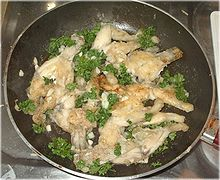
\includegraphics[width = .5\textwidth]{cuisine/miam.JPG}
				\caption{Cuisses de grenouilles}
				\label{fig:gre}
		\end{center}
	\end{figure}

				
\end{document}